Folgender Kapitel betrachtet der physikalische Vorgang  einer im zeitlichen Mittel konstanten Ladungsträgerbewegung. Hiermit wird das Ohmsche Gesetz, Energie und Leistung eines stationären Strömungsfeld durch die Stromdichte und die elektrischer Feldstärke. Randbedingungen an Materialsprungstellen werden noch behandelt.
%%%%%%%%%%%%%%%%%%%%%%%%%%%%%%%%%%%%%%%%%%%%%%%%%%%%%%%%%%%%%%%%%%%%%%%%%%%%%%%%%%%%%%%%%%%%%%%%
\section{Der elektrische Strom}
Auf zwei geladenen Körpern namens \textbf{Elektroden} befinden sich die entgegengesetz gleichen Gesamtladungen $+Q$ und $-Q$. Die Elektrode 1 mit Ladung $+Q$ besitzt das Potential $\varphi_{e1}$ und die Elektrode 2 mit Ladung $-Q$ das Potential $\varphi_{e2}<\varphi_{e1}$.
\begin{figure}[H]
\frame{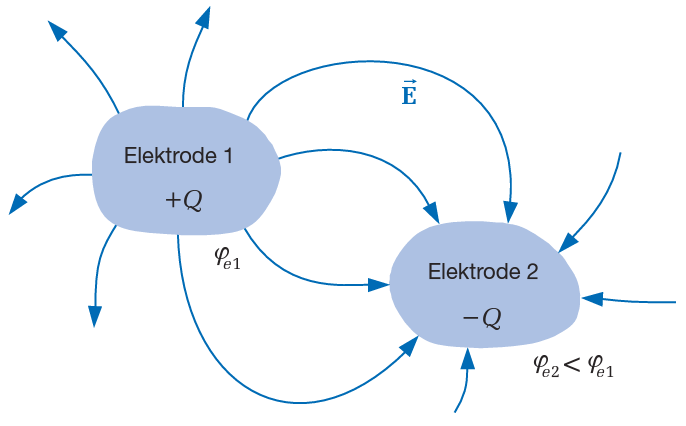
\includegraphics[scale=0.5]{../img/II/IIa}}
\centering
\caption{Zwei Elektroden mit entgegengesetzt gleichen Ladungen.}
\label{fig_IIa}
\end{figure}
\noindent Die elektrische Feldlinien verlaufen von den positiven Ladungen der Elektrode 1 zu den negativen Ladungen der Elektrode 2. Zwischen den Elektroden besteht die Spannung $U_{12}$ aus der Differenz der Potentiale beider Elektroden.
\begin{equation}
\boxed{U_{12}=\varphi_{e1}-\varphi_{e2}}
\end{equation}
Mit Hilfe eines Drahtes stellt man eine leitende Verbindung zwischen den beiden Elektroden her, in der sich die Elektronen frei bewegen können. Die wirkende Kraft auf die Ladungsträger führt dazu, dass ein Ladungsausgleich zwischen den beiden Elektroden stattfindet. Dieser Vorgang ist dann beendet, wenn im Draht zwischen den Elektroden keine elektrische Feldstärke, d.h. zwischen ihnen keine Spannung mehr vorhanden ist. Beide Elektroden besitzen in diesem Endzustand das gleiche Potential.
\begin{figure}[H]
\frame{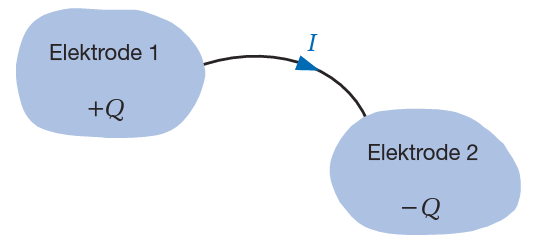
\includegraphics[scale=0.5]{../img/II/IIb}}
\centering
\caption{Ladungsträgerbewegung zwischen Elektroden unterschiedlichen Potentials.}
\label{fig_IIb}
\end{figure}
\noindent Die Bewegung der Ladungsträger bezeichnet man als \textbf{elektrischen Strom}. Die Richtung eines positiven Stromes ist so definiert, dass er von der Elektrode höheren Potentials zur Elektrode niedrigeren Potentials fliesst. Er hat damit innerhalb der leitenden Verbindung die gleiche Richtung wie die elektrische Feldstärke.
\newline\newline
Die negativen Ladungsträger (Elektronen) bewegen sich entgegengesetzt zur festgelegten Stromrichtung, d.h. von der Elektrode niedrigeren Potentials zur Elektrode höheren Potentials. Den durch einen Transport von Ladungsträgern verursachten Strom nennt man \textbf{Konvenktionsstrom}. Im Gegensatz dazu tritt bei zeitabhängigen Vorgängen der so genannte \textbf{Verschiebungsstrom} auf, der proportional zur zeitlichen Ableitung der Verschiebungsdichte $\partial \overrightarrow{D}/\partial t$ ist.
\newline\newline
An einer beliebigen Stelle der leitenden verbindung betrachtet man deren gesamte Querschnittsfläche. Während eines kleinen Zeitabschnittes $\triangle t$ erfasst man alle Ladungsträger, die diese Querschnittsfläche in einer bestimmten Richtung durchströmt. Das Produkt aus der Summe dieser Ladungsträger und dem Wert der Elementarladung stellt eine \textbf{Ladungsmenge} dar, die man mit $\triangle Q$ bezeichnet. In der Zeitspanne $\triangle t$ während des Ausgleichsvorgangs fliesst durch die leitende Verbindung von der Elektrode 1 zur Elektrode 2 die Ladungsmenge $\triangle Q$. 
\newline \newline
Das Verhältnis aus der transportierten Ladungsmenge $\triangle Q$ und der betrachteten Zeit $\triangle t$ bezeichnet man als \textbf{Stromstärke} $I$ und hat Dimension A. Die \textbf{mittlere Stromstärke} in dem betrachteten Zeitabschnitt $\triangle t$ lautet
\begin{equation}
\boxed{I=\dfrac{\triangle Q}{\triangle t}}
\end{equation}
Interessiert man sich für den Wert der Stromstärke in einem Augenblick zu einen beliebigen Zeitpunkt $t$, dann muss man die Dauer des Zeitabschnitts $\triangle t$ gegen Null gehen lassen und zwar so, dass der Zeitpunkt $t$ immer innerhalb von $\triangle t$ verbleibt. Sie Stromstärke in dem betrachteten Zeitpunkt lässt sich dann als Differentialquotient schreiben.
Die \textbf{momentane Stromstärke} bei einem beliebigen Zeitpunkt $t$ lautet
\begin{equation}
\boxed{I\left(t\right)=\displaystyle \lim_{\triangle t\rightarrow 0}\dfrac{\triangle Q}{\triangle t}=\dfrac{\text{d}Q}{\text{d}t}}
\end{equation}
Die obigen Gleichungen enthalten keine Information über die örtliche Verteilung der Ladungsträgerbewegung innerhalb der leitenden Verbindung.
%%%%%%%%%%%%%%%%%%%%%%%%%%%%%%%%%%%%%%%%%%%%%%%%%%%%%%%%%%%%%%%%%%%%%%%%%%%%%%%%%%%%%%%%%%%%%%%%
\section{Die Stromdichte}
Zwischen zweier Elektroden besteht der Raum aus einem leitfähigen Material. Der von einer Elektrode 1 zur Elektrode 2 fliessende Gesamtstrom $I$ wird sich mit einer ortsabhängigen \textbf{Dichte} über den gesamten Raum verteilen. 
\newline\newline
Um die Elektrode 1 legt man eine geschlossene Hüllfläche $A$. So soll $A$ gewählt sein, dass die Bewegungsrichtung der Ladungsträger an jeder Stelle senkrecht zur Hüllenfläche verläuft. Somit sei der Winkel $\alpha$ zwischen der Ladungsträgerbewegung in Richtung $\overrightarrow{J}$ und der Flächennormalen $\overrightarrow{n}$ überall Null. Durch ein elementares Flächenelement $\triangle A$ wird der elementare Anteil des Stromes $\triangle I$ hindurchtreten. 
\begin{figure}[H]
\frame{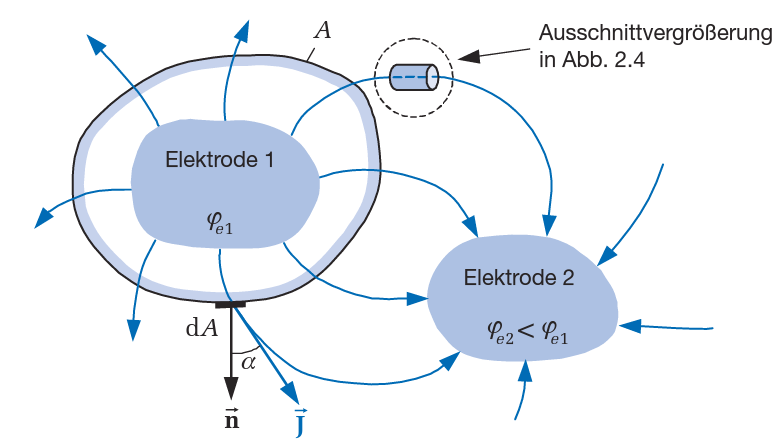
\includegraphics[scale=0.5]{../img/II/IIc}}
\centering
\caption{Räumlich verteilter Stromfluss zwischen Elektroden unterschiedlichen Potentials.}
\label{fig_IIc}
\end{figure}
\noindent Das Verhältnis aus elementarem Stromanteil und elementarem Flächenelement nennt man \textbf{Stromdichte} und hat Dimension Am$^{-2}$.
\begin{equation}
\boxed{J=\dfrac{\triangle I}{\triangle A}}
\end{equation}
\noindent Schneidet man aus dem stromführenden Bereich zwischen den beidenElektroden ein elementares Volumenelement mit den Stirnseiten $\triangle A$ und der Mantelfläche $M$ heraus. Das Volumenelement sei so gewählt, dass sichdie Ladungsträger parallel zur Mantelfläche bewegen und seine Länge sei so klein, dass sich die Querschnittsfläche $\triangle A$ längs der Abmessung $\triangle x$ nicht ändert.
\begin{figure}[H]
\frame{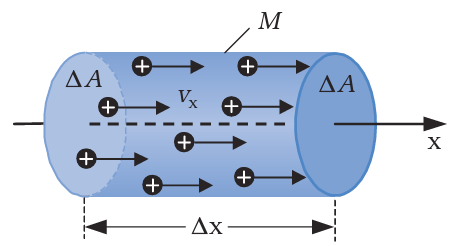
\includegraphics[scale=0.6]{../img/II/IId}}
\centering
\caption{Bewegung einer Raumladung in $x$-Richtung.}
\label{fig_IId}
\end{figure}
\noindent Sei die $x$-Achse eines Koordinatensystems parallel zur Bewegungsrichtung der Ladungsträger eingeführt. Bewegen sich die Ladungsträger mit der \textbf{Geschwindigkeit} $v_x$, dann benötigen sie zum Durchlaufen einer Strecke $\triangle x$ die Zeit $\triangle t$.
\begin{equation}
\boxed{\triangle x=v_x\cdot \triangle t}
\end{equation}
In einem Zeitabschnitt $\triangle t$ werden diejenige Ladungsträger die rechte Stirnseite der Stromröhre durchfliessen, die sich zum Beginn des Beobachtungszeitraumes innerhalb der Stromröhre mit der Länge $\triangle x$ befinden. Das Volumenelement $\triangle V$ entsteht aus der Ladungsmenge $\triangle Q$ mit dem \textbf{mittleren Raumladungsdichte} $\rho$. Dann entspricht die $x$-gerichtete \textbf{Stromdichte} $J_x$
\begin{equation}
\boxed{\triangle Q=\rho\cdot \triangle V}\quad \boxed{\triangle V=\triangle A\cdot \triangle x}
\end{equation}
\begin{equation}
\boxed{J_x=\dfrac{\triangle I}{\triangle A}=\dfrac{\triangle Q}{\triangle A\cdot \triangle t}=\dfrac{\triangle Q}{\triangle V}\dfrac{\triangle x}{\triangle t}=\rho\cdot v_x}
\end{equation}
Eine grössere Stromdichte kann entweder durch eine grössere Anzahl der am Ladungsträgertransport beteiligten Elementarladungen im Volumen oder durch eine höhere Geschwindigkeit zustande kommen.
\newline\newline 
Im dreidimensionalen Fall durch den Geschwindigkeitsvektor $\overrightarrow{v}=v_x\overrightarrow{e}_x+v_y\overrightarrow{e}_y+v_z\overrightarrow{e}_z$ ist die Stromdichte
\begin{equation}
\boxed{\overrightarrow{J}=\rho\cdot \overrightarrow{v}=\left(-\rho\right)\cdot \left(-\overrightarrow{v}\right)}
\end{equation}
Bei \textbf{positiven Raumladung} ($\rho>0$) zeigen Stromdichte $\overrightarrow{J}$ und Geschwindigkeit $\overrightarrow{v}$ in die gleiche Richtung. Bei einer \textbf{negativen Raumladung} ($\rho<0$) zeigt die Kraft auf die Ladungsträger in die entgegengesetzte Richtung, so dass sich die Bewegungsrichtung und damit auch das Vorzeichen von $\overrightarrow{v}$ ebenfalls umkehrt. Das Produkt ist für beide Ladungsträgerarten gleich.
\newline\newline
Betrachtet man wieder die \textbf{\textit{Abbildung \ref{fig_IId}}} eine beliebig geformte Hüllfläche $A$, mit der senkrecht auf der Fläche stehenden Flächennormalen $\overrightarrow{n}$ der Länge $\Big\vert\overrightarrow{n}\Big\vert=1$ und erweitert man das skalare Flächenelement $\text{d}A$ auf das vektorielle Flächenelement $\text{d}\overrightarrow{A}=\overrightarrow{n}\text{d}A$, das mit der an dem Ort des Flächenelements vorliegenden Stromdichte $\overrightarrow{J}$ den Winkel $\alpha$ einschliesst. Den elementaren Strom durch $\text{d}A$ erhält man aus der Multiplikation von $\text{d}A$ mit der senkrecht zu $\text{d}A$ stehenden Komponente der Stromdichte $\overrightarrow{J}$ bzw. aus dem Skalarprodukt der beiden Vektoren
\begin{equation} 
\boxed{\text{d}I=\Big\vert\overrightarrow{J}\Big\vert\cdot \text{d}A\cdot \cos\left(\alpha\right)=\overrightarrow{J}\bullet\text{d}\overrightarrow{A}}
\end{equation} 
Zur Berechnung des Gesamtstromes durch eine Fläche $A$ müssen die Beiträge über die Fläche integriert werden
\begin{equation}
\boxed{I=\displaystyle \iint_{A}\overrightarrow{J}\bullet \text{d}\overrightarrow{A}} 
\end{equation} 
Soll der Strom zwischen den Elektroden unabhängig von der Zeit immer einen konstanten Wert aufweisen, dann müssen die von den Elektroden abfliessenden Ladungsträger immer wieder nachgeliefert werden. Da die Ladungsträger weder erzeugt noch vernichtet werden können, ist im stationären Zustand die innerhalb eines umschlossenen Volumens vorhandene Summe der Ladungsträger zeitlich konstant und das obige Integral über eine geschlossene Fläche verschwindet.
\begin{equation}
\boxed{I=\displaystyle \oiint_{A}\overrightarrow{J}\bullet \text{d}\overrightarrow{A}=0}
\end{equation}
%%%%%%%%%%%%%%%%%%%%%%%%%%%%%%%%%%%%%%%%%%%%%%%%%%%%%%%%%%%%%%%%%%%%%%%%%%%%%%%%%%%%%%%%%%%%%%%%
\section{Ladungsträgerbewegung im Leiter}
Ladungsträger können sich in einem Material zwischen den beiden Elektroden bewegen. Bei Metallen sind die Elektronen auf der äusseren Schale praktisch ungebunden. Sie können sich relativ frei innerhalb des Atomverbandes bewegen. Ein Material mit frei beweglichen Elektronen bezeichnet man als \textbf{Leiter}. Die positiven Ladungsträger (Protonen) sind dagegen ortsfest. In einem Metal bewegen sich die Elektronen ohne äussere Einflüsse ungeordnet zwischen den Atomen hin und her. Da sie sich mit gleicher Wahrscheinlichkeit in jede Richtung bewegen können, verschwindet der über alle Elektronen gebildete Mittelwert ihrer Bewegungen.
\newline\newline
Ein \textbf{Konvenktionsstrom} ist nach aussen nicht feststellbar. Diese Situation ändert sich, wenn eine elektrische Feldstärke $\overrightarrow{E}$ vorhanden ist. Die Elektronen erfahren als negative Ladungsträger nach dem Coulomb'schen Gesetz eine Kraft, die entgegengesetzt zur elektrischen Feldstärke gerichtet ist. Ihrer bisherigen stückweise geradlinigen Bewegung ist eine permanente Beschleunigung in eine von der Feldstärke aufgeprägte Richtung überlagert.
\newline\newline
Diese beschleunigte Bewegung wird immer wieder unterbrochen durch Zusammenstösse, einerseits mit den ortsfesten Atomen im Gitter und andererseits infolge der Unregelmässigkeiten im Gitteraufbau. Dabei werden die Elektronen an den Stossstellen sowohl gestreut, d.h. ihre Bewegungsrichtung ändert sich, als auch abgebremst, wobei sie ihre kinetische Energie zum Teil verlieren.
\newline\newline
Die fortwährend erneute Beschleunigung verleiht den Elektronen im Mittel aber eine so genannte \textbf{Driftgeschwindigkeit} $\overrightarrow{v}_e$, die proportional zum Betrag der elektrischen Feldstärke ist. Den Proportionalitätsfaktor $\mu_e$ zwischen der Driftgeschwindigkeit und der Feldstärke bezeichnet man als \textbf{Beweglichkeit}. Das Minuszeichen bringt die unterschiedlichen Richtungen der beiden Vektoren, nämlich der Feldstärke und der ihr entgegengesetzt gerichteten Elektronenbewegung. Die Beweglichkeit $\mu_e$ ist eine positive Grösse.
\begin{equation}
\boxed{\overrightarrow{v}_e=-\mu_e\cdot \overrightarrow{E}}
\end{equation}
Angenommen die elektrische Feldstärke sei $x$-gerichtet, dann legen die Elektronen in einem endlichen Zeitintervall $\triangle t$ einen mittleren Weg $\triangle s$ in negativer $x$-Richtung zurück. Verlässt ein Elektron sein Atom, dann entsteht ein als \textbf{Ion} bezeichnetes positiv geladenes Atom. Wird diese freigewordene Stelle von einem nachrückenden Elektron besetzt, dann haben sich nicht nur Elektronen entgegen der Feldstärkerichtung bewegt, sondern die frei werdenden Stellen bewegen sich in Richtung der Feldstärke.
%%%%%%%%%%%%%%%%%%%%%%%%%%%%%%%%%%%%%%%%%%%%%%%%%%%%%%%%%%%%%%%%%%%%%%%%%%%%%%%%%%%%%%%%%%%%%%%%
\section{Die spezifische Leitfähigkeit und der spezifische Widerstand}
Mit folgenden Gleichungen wird einen Zusammenhang zwischen der Stromdichte $\overrightarrow{J}$ und der elektrischen Feldstärke $\overrightarrow{E}$ erzeugt.
\begin{equation}
\boxed{\overrightarrow{J}=\rho\cdot \overrightarrow{v}}\quad \boxed{\overrightarrow{v}_e=-\mu_e\cdot \overrightarrow{E}}
\end{equation}
Bezeichnet man mit $n$ die \textbf{Ladungsträgerkonzentration}, d.h. die Anzahl der freien Elektronen pro Volumen, dann gilt mit der \textbf{Raumladungsdichte} $\rho=-n\cdot e$ und der \textbf{Driftgeschwindigkeit} $\overrightarrow{v}_e$ der Elektronen die Beziehung
\begin{equation}
\boxed{\overrightarrow{J}=\left(-n\cdot e\right)\cdot \overrightarrow{v}_e=n\cdot e\cdot \mu_e\cdot \overrightarrow{E}=\kappa\cdot \overrightarrow{E}}
\end{equation}
Die Abkürzung $\kappa$ wird als \textbf{spezifische Leitfähigkeit} bezeichnet und hat die Dimension ${\mathrm{\Omega}}^{-1}\text{m}^{-1}$. In vielen Fällen wird anstelle der spezifischen Leitfähigkeit deren Kehrwert verwendet. Diese als \textbf{spezifischer Widerstand} $\rho_R$ bezeichnete Materialeigenschaft ist zusammen mit der spezifischen Leitfähigkeit für verschiedene Materialien angegeben. Der Index $R$ (resistivity) wird hier verwendet, um Verwechselungen mit der mit gleichem Buchstaben bezeichneten Raumladungsdichte zu vermeiden. Aus technischen Gründen wird vielfach nicht die Einheit ${\mathrm{\Omega}}\text{m}$, sondern ${\mathrm{\Omega}}\text{mm}^{2}\text{m}^{-1}$, verwendet.
\begin{equation}
\boxed{\rho_R=\dfrac{1}{\kappa}}
\end{equation}
In der Praxis lässt sich eine Abhängigkeit des spezifischen Widerstandes von der Temperatur feststellen. In den meisten technischen Anwendungen ist der auftretende Temperaturbereich soweit begrenzt, dass die Temperaturabhängigkeit $\rho_R\left(\theta\right)$ durch eine lineare Näherung hinreichend genau beschrieben werden kann. Mathematisch stellt man dieen Zusammenhang durch folgende Gleichung dar
\begin{equation}
\boxed{\rho_R\left(\theta\right)=\rho_{R,20^{\circ}\text{C}}\cdot \Big[1+\alpha\left(\theta-20^{\circ}\text{C}\right)\Big]=\rho_{R,20^{\circ}\text{C}}\cdot\left(1+\alpha\triangle \theta\right)}
\end{equation}
Darin beschreibt $\rho_{R,20^{\circ}\text{C}}$ den angegebenen spezifischen Widerstand bei der Umgebungstemperatur $\theta_u=20^{\circ}\text{C}$ und der Temperaturkoeffizient $\alpha$ beschreibt den linearen Anstieg des spezifischen Widerstandes mit der Temperatur $\theta$.
\newline\newline
Eine noch bessere Beschreibung der Temperaturabhängigkeit lässt sich erreichen, wenn in der obigen Beziehung ein weiterer Korrekturfaktor hinzugefügt wird, der sich quadratisch mit der Temperatur ändert und die Abweichung des temperaturabhängigen spezifischen Widerstandes von dem linearen Verlauf beschreibt.
\begin{equation}
\boxed{\rho_R\left(\theta\right)=\rho_{R,20^{\circ}\text{C}}\cdot\Big[1+\alpha\triangle \theta+\beta\left(\triangle \theta\right)^2\Big]}
\end{equation}
Die \textbf{Temperaturabhängigkeit des spezifischen Widerstandes} wird von verschiedenen Faktoren beeinflusst. Betrachte man uinächst die Metalle mit ihrem relativ regelmässigen Gitteraufbau. Die Beweglichkeit der freien Elektronen ist abhängig von der mittleren freien Weglänge zwischen zwei Zusammenstössen. Der Wert für die Beweglichkeit $\mu_e$ wird geringer mit abnehmender freier Weglänge. In Abhängigkeit von der Temperatur schwingen die Atome um ihre feste Gleichgewichtslage und zwar umso mehr, je höher die Temperatur wird. 
\newline\newline
Die Wahrscheinlichkeit der Stösse nehmen durch steigender Temperatur zu, die mittlere freie Weglänge wird kürzer und der spezifische Widerstand steigt an. Der Temperaturkoeffizient $\alpha$ ist daher positiv und liegt bei allen reinen Metallen in ähnlicher Grossenanordnung.
\newline\newline
Bei \textbf{Legierungen} führt der unregelmässige Gitteraufbau zu einer erhöhten Wahrscheinlichkeit für Zusammenstösse der Elektronen mit den Gitteratomen. Der spezifische Widerstand ist bei Legierungen daher wesentlicher grösser. Gleichzeitig spielt der Einfluss der thermischen Gitterschwingungen auf die Anzahl der Zusammenstösse nur noch eine untergeordnete Rolle, so dass der Temperaturkoeffizient deutlich geringer ist. Solche Legierungen werden bevorzugt benutzt zur Herstellung temperaturabhängiger Präzisionswiderstände.
\newline\newline
Bei \textbf{Halbleitern} nimmt die Beweglichkeit $\mu_e$ der freien Ladungsträger mit steigender Temperatur zwar ebenfalls ab, ihre Zahl pro Volumen steigt aber an, so dass die Leitfähigkeit dennoch zunimmt und der Temperaturkoeffizient einen negativen Zahlenwert besitzt. 
%%%%%%%%%%%%%%%%%%%%%%%%%%%%%%%%%%%%%%%%%%%%%%%%%%%%%%%%%%%%%%%%%%%%%%%%%%%%%%%%%%%%%%%%%%%%%%%%
\section{Das Ohm'sche Gesetz}
Der Zusammenhang zwischen der Stromdichte $\overrightarrow{J}$ und der elektrischen Feldstärke $\overrightarrow{E}$ wird als \textbf{Ohm'sches Gesetz }bezeichnet. Diese Gleichung beschreibt den Zusammenhang zwischen der im allgemeinen Fall dreidimensionalen Stromdichteverteilung und der zugehörigen Feldstärkeverteilung an jeder Stelle des Raumes. Die elektrische Feldstärke im stromdurchflossenen Leiter besitzt einen nicht verschwindenden Wert.
\begin{equation}
\boxed{\overrightarrow{J}=\kappa\cdot \overrightarrow{E}}
\end{equation}
Die Stromdichte kann sich aus drei verktoriellen Komponenten zusammensetzen, die ihrerseits wiederum von allen drei Koordinaten abhängen können. In manchen Fällen ist diese aufwändige Berechnung der Strömungsfelder unumgänglich, sehr häufig ist jedoch die Beschreibung und Lösung eines Problems mit integralen Grössen ausreichend.
\newline\newline
Betrachte ein zylindrischer Leiter der Länge $l$ und der Querschnittsfläche $A$ aus einem homogenen Material der Leitfähigkeit $\kappa$. Die beiden Stirnseiten befinden sich auf den Potentialen $\varphi_{e1}$ und $\varphi_{e2}<\varphi_{e1}$ und spielen die gleiche Rolle wie die beide Elektroden. Nimmt man an dass die beiden Elektroden aussen an eine Quelle angeschlossen werden, die die abfliessenden Ladungsträger immer wieder nachliefert, dann wird von der Elektrode höheren Potentials ein Gleichstrom $I$ zu der Elektrode mit niedrigerem Potential fliessen, der sich aus Symmetriegründen gleichmässig über den Leiterquerschnitt verteilt. Damit gilt
\begin{equation}
\boxed{\overrightarrow{J}=J_x\cdot \overrightarrow{e}_x=\dfrac{I}{A}\cdot \overrightarrow{e}_x}
\end{equation}
\begin{figure}[H]
\frame{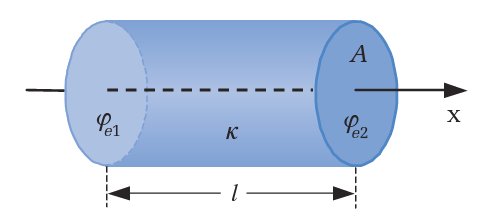
\includegraphics[scale=0.6]{../img/II/IIe}}
\centering
\caption{Widerstand eines zylindrischen Leiters.}
\label{fig_IIe}
\end{figure}
\noindent Aus dem Ohm'schen Gesetz ist die \textbf{elektrische Feldstärke} innerhalb des Leiters 
\begin{equation}
\boxed{\overrightarrow{E}=E_x\cdot \overrightarrow{e}_x=\dfrac{\overrightarrow{J}}{\kappa}=\dfrac{J}{\kappa}\cdot \overrightarrow{e}_x=\dfrac{1}{\kappa}\dfrac{I}{A}\cdot \overrightarrow{e}_x}
\end{equation}
Drückt man die zwischen den Elektroden anliegende Spannung durch das Wegintegral der Feldstärke aus, dann erhält man einen Zusammenhang zwischen der anliegenden Spannung und dem insgesamt fliessenden Strom.
\begin{equation}
\boxed{
\begin{array}{lll}
U_{12}=\varphi_{e1}-\varphi_{e2}&=&\displaystyle \int_{P_1}^{P_2}\overrightarrow{E}\bullet \text{d}\overrightarrow{s}=\displaystyle \int_{x=0}^l\dfrac{1}{\kappa}\dfrac{I}{A}\cdot \overrightarrow{e}_x\bullet \overrightarrow{e}_x\text{d}x\\
&=&\dfrac{I}{\kappa \cdot A}\displaystyle \int_{x=0}^l\text{d}x=\dfrac{I\cdot l}{\kappa\cdot A}
\end{array}
}\quad 
\boxed{U_{12}=R\cdot I}
\end{equation}
\begin{equation}
\boxed{R=\dfrac{l}{\rho\cdot A}=\dfrac{\rho_R\cdot l}{A}}
\end{equation}
Der Proportionalitätsfaktor $R$ heisst \textbf{elektrischer Widerstand} und hat die Dimension VA$^{-1}=\Omega$. Der Widerstand des betrachteten Zylinders ist durch die obige Beziehung definiert. Der Widerstand ist von der Geometrie der Anordnung und von den Materialeigenschaften abhängig.
\newline\newline
Für den spezifischen Widerstand $\rho_R$ des Materials in Funktion der Temperatur gilt analog für den Widerstand
\begin{equation}
\boxed{R\left(\theta\right)=\rho_R\left(\theta\right)\cdot \dfrac{l}{A}=\rho_{R,20^{\circ}C}\cdot \left(1+\alpha\cdot \triangle \theta\right)\cdot \dfrac{l}{A}=R_{20^{\circ}C}\cdot \left(1+\alpha\cdot \triangle \theta\right)}
\end{equation}
Die Spannung $U_{12}$ ist noch mit den beiden Indizes 12 behaftet, die die Zählrichtung der Spannung von der Elektrode 1 mit höherem Potential zu der Elektrode 2 mit niedrigerem  Potential zum Ausdruck bringen. Da der Strom aber in der gleichen Richtung positiv gezählt wird, kann auf die beiden Indizes verzichtet werden. Daraus entsteht folgende Beziehungen
\begin{equation}
\boxed{U=R\cdot I}
\end{equation}
\begin{equation}
\boxed{I=\displaystyle \iint_{A}\overrightarrow{J}\bullet\text{d}\overrightarrow{A}=\kappa\displaystyle \iint_{A}\overrightarrow{E}\bullet \text{d}\overrightarrow{A}}\quad \boxed{U=\displaystyle \int_s\overrightarrow{E}\bullet \text{d}\overrightarrow{s}}\quad \boxed{R=\dfrac{U}{I}=\dfrac{\displaystyle \int_s\overrightarrow{E}\bullet \text{d}\overrightarrow{s}}{\kappa\displaystyle \iint_{A}\overrightarrow{E}\bullet \text{d}\overrightarrow{A}}}
\end{equation}
Das Strom-Spannungs-Diagramm erzeugt eine Gerade, deren Steigung $\triangle I/\triangle U$ dem Kehrwert des Widertandes entspricht. Ein grösserer Widerstand bedeutet eine geringere Steigung. Bei einer Temperatur von $20^{\circ}C$ hat einen Kupferdraht den Widerstand von $1\Omega$. Der gleiche Kupferdrht hat bei $100^{\circ}C$ einen Widerstand von 1.31$\Omega$.
\begin{figure}[H]
\frame{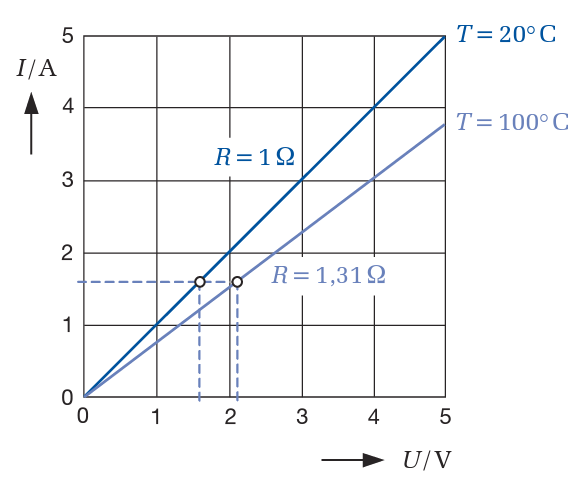
\includegraphics[scale=0.6]{../img/II/IIf}}
\centering
\caption{Widerstandsgerade eines Kupferdrahtes bei unterschiedlichen Temperaturen.}
\label{fig_IIf}
\end{figure}
\noindent Die zugehörige Widerstandsgerade im Strom-Spannungs-Diagramm hat jetzt einen flächeren Verlauf, d.h. bei gleichem Strom durch den Kupferdraht nimmt der Spannnungsabfall entlang des Drahtes mit steigender Temperatur zu. Wird dagegen die an den Draht angelegte Spannung konstant gehalten, dann fliesst bei niedrigerer Temperatur wegen des geringeren Widerstandes ein grösserer Strom.
\newline\newline
In vielen Fällen wird die Berechnung von Schaltungen dadurch erleichtert, dass man nicht den Widerstand, sondern seinen Kehrwert verwendet. 
\begin{equation} 
\boxed{G=\dfrac{1}{R}}
\end{equation}
$G$ heisst \textbf{elektrischer Leitwert} des Widerstands und besitzt die Dimension AV$^{-1}=\Omega^{-1}$.
\section{Praktische Ausführungsformen von Widerstände}
Neben dem Widerstandswert sind insbesondere die Herstellungstoleranz, die Temperaturabhängigkeit des Widerstandes, die maximal zulässige Verlustleistung, die Kurzzeitbelastung oder der Dauerbetrieb von besonderer Bedeutung.
\subsection{Festwiderstände}
Die \textbf{Festwiderstände} haben eine lineare Widerstandscharakteristik und genügen dem Ohm'schen Gesetz. Die Abstufung der Widerstandtswerte entspricht den in den Normen festgelegtem E-Reihen. Die spezielle Kennzeichnung einer E-Reihe durch den betreffenden Zahlenwert gibt an, wie viele Werte innerhalb jeder Dekade liegen. Festwiderstände werden als \textbf{Schicht-}, \textbf{Draht-} oder \textbf{Massewiderstände} hergestellt. 
\newline\newline
Bei den \textbf{Schichtwiderständen} wird eine dünne Widerstandsschicht aus Kohle oder Metall auf einen zylindrischen Träger aus Keramik oder Glas aufgebracht. An den Enden werden Kappen aufgepresst und mit den Anschlüssen versehen. Zum Schutz wird das Bauelement mit einer Schicht aus Lack oder Kunststoffüberzogen. Zur Herstellung grösserer Widerstandswerte wird die dünne Metall- oder Kohleschicht gewendelt ausgeführt. 
\newline\newline
Bei höheren Leistungen werden \textbf{Drahtwiderstände} eingesetzt, bei denen der Träger mit einem Draht umwickelt wird. Kleine Widerstandswerte können auf diese Weise leicht hergestellt werden, bei grösseren Werten wird spezieller Widerstandsdraht verwendet. Der Drahtquerschnitt begrenzt den maximal zulässigen Strom und die maximale Verlustleistung wird durch die Wärmeabfuhr, d.h. die Bauteilgrösse und die Ausführung der Oberfläche bestimmt. Zur Reduzierung parasitären Induktivitäten werden die Wicklungen \textbf{bifilar} ausgeführt, d.h. es werden zwei Drähte so nebeneinander gewickelt, dass sie in entgegengesetzter Richtung vom Strom durchflossen werden. Eine weitere Möglichkeit zur Reduzierung der parasitären Induktivitäten besteht darin, den Wickelsinn mehrfach umzudrehen.
\newline\newline
Die \textbf{Massenwiderstände} besitzen keinen Träger, sondern bestehen insgesamt aus einem Widerstandsmaterial. Sie werden in verschiedenen Bauformen, bpsw. als Stäbe oder Scheiben, hergestellt.
\begin{figure}[H]
\frame{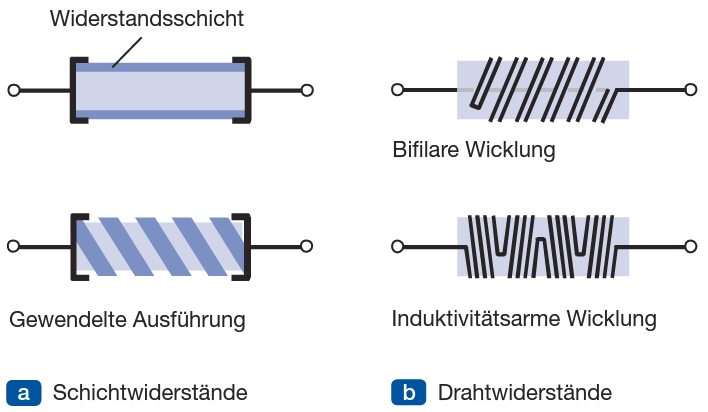
\includegraphics[scale=0.6]{../img/II/IIg}}
\centering
\caption{Bauformen von Festwiderständen.}
\label{fig_IIg}
\end{figure}
\subsection{Einstellbare Widerstände}
Bei einstellbaren Widerständen wird ein Schleifkontakt über das nicht isolierte Widerstandsmaterial bewegt. Bei einem \textbf{Schiebewiderstand} ist der Wickelkörper linear gestreckt, bei einem \textbf{Drehwiderstand} dagegen ringförmig ausgeführt. Üblichwerweise spricht man bei diesen Bauelementen von \textbf{Potentiometern}, wenn sie im Betrieb immer wieder neu eingestellt werden, bzw. von \textbf{Trimmpotentiometern}, wenn sie nur einmal, zum Abgleich einer Schaltung auf einen bestimmten Wert justiert werden.
\subsection{Weitere Widerstände}
Für besondere Aufgaben gibt es eine grosse Gruppe von nichtlinearen Widerständen, deren Verhalten von unterschiedlichen physikalischen Grössen abhängen kann.
\newline\newline
Zu der \textbf{temperaturabhängigen Widerstände} gehören die \textbf{Heissleiter}, deren Widerstand mit steigender Temperatur kleiner wird. Sie werden als \textbf{NTC} (negative temperature coefficient) bezeichnet. Diese Bauelemente besitzen bei Raumtemperatur einen grosseren Widerstand und begrenzen beim Einschalten eines elektronischen Gerätes dessen Einschaltstrom. Infolge der ohmschen Verluste werden sie stark aufgeheizt, wodurch ihr Widerstand sehr viel kleiner wird. Im Dauerbetrieb einer Schaltung verursachen sie dann lediglich geringe Verluste. Das temperaturabhängige Verhalten ist bei den als \textbf{PTC} (positive temperature coefficient) bezeichneten \textbf{Kaltleitern} genau umgekehrt.
\newline\newline
Widerstände, deren Wert von der Spannung abhängt, werden als \textbf{VDR} (voltage dependent resistor) bezeichnet. Sie werden zur Spannungsstabilisierung oder zur Unterdrückung von kurzzeitigen Spannungsspitzen eingesetzt.
\newline\newline
Eine weitere Gruppe sind die als \textbf{LDR} (light dependent resistor) bezeichneten lichtabhängigen Widerstände, die für Belichtungsmesse oder bei helligkeitsabhängigen Steuerungen verwendet werden.
\section{Energie und Leistung}
Bei dem Stromleitungsmechanismus der Driftbewegung werden die Elektronen durch das anliegende Feld beschleunigt. Die Zunahme der kinetischen Energie wird dem Energieinhalt des elektrischen Feldes entnommen. Bezeichnet man mit $\triangle Q$ die transportierte elementare Ladung, dann ist die dem Feld entnommene elementare Energie $\triangle W_e$ aus dem Produkt der Ladung und der durchlaufenen Potentialdifferenz gegeben. Damit gilt der Zusammenhang
\begin{equation}
\boxed{\triangle W_e=\left(\varphi_{e1}-\varphi_{e2}\right)\cdot \triangle Q=U\cdot \triangle Q=U\cdot I\cdot \triangle t}
\end{equation}
Die dem Feld entnommene Energie nimmt einen positiven Wert an, wenn bspw. eine positive Ladung $\triangle Q$ von einem höheren Potential $\varphi_{e1}$ zu einem niedrigeren potential $\varphi_{e2}$ bewegt wird. Das Verhältnis aus geleisteter Arbeit $\triangle W_e$ und dazu benötigter Zeit $\triangle t$ wird allgemein als \textbf{Leistung} bezeichnet und mit $P$ abgekürzt.
\begin{equation}
\boxed{P=\dfrac{\triangle W_e}{\triangle t}=U\cdot I}
\end{equation}
Bei den zeitlich konstanten Grössen Gleichspannung $U$ und Gleichstrom $I$ ist auch die Leistung $P$ zeitlich konstant und somit unabhängig von der Wahl des elementaren Zeitabschnitts $\triangle t$. Sind dagegen Strom und Spannung zeitlich veränderliche Grössen, dann beschreibt $P$ lediglich dem Mittelwert der Leistung in den beiden betrachteten Zeitintervall. Interessiert man sich bei einem bestimmten Zeitpunkt $t$, dann muss man den Zeitabschnitt $\triangle t$ gegen Null gehen lassen und zwar so, dass der Zeitpunkt $t$ immer innerhalb von $\triangle t$ verbleibt. Die Leistung in dem betrachteten Zeitpunkt lässt sich dann als Differentialquotient in der Form schreiben. Die Leistung hat die Dimension VA$=$W. Die elektrische Arbeit hat die Dimension kWh.
\begin{equation}
\boxed{P\left(t\right)=\displaystyle \lim_{\triangle t\rightarrow 0}\dfrac{\triangle W_e}{\triangle t}=\dfrac{\text{d}W_e}{\text{d}t}}\quad \boxed{W_e=\displaystyle \int_tP\left(\tau\right)\,\text{d}\tau}
\end{equation}
Die berechnete Leistung wird an dem Widerstand in Wärme umgewandelt. Mit dem Ohm'schen Gesetz kann die Leistung an einem Widerstand $R$ auch in der Form geschrieben werden. Da sowohl der Strom als auch die Spannung quadratisch auftreten, spielt ihre Zählrichtung keine Rolle. Der Wert von $P$ beschreibt die an einem Widerstand $R$ entstehende \textbf{Verlustleistung}.  
\begin{equation}
\boxed{
\begin{array}{lll}
P&=&U\cdot I=\left(R\cdot I\right)\cdot I=R\cdot I^2\\
&=&U\cdot I=U\cdot \dfrac{U}{R}=\dfrac{U^2}{R}
\end{array}}
\end{equation}
Bei vielen Problemstellungen fragt man sich nach der \textbf{örtlichen Verteilung} der in einem Volumen entstehenden Verluste. Zur Beantwortung dieser Frage betrachtet man das elementare Volumenelement $\triangle V=\triangle A\cdot \triangle x$. Dei Querschnittsfläche $\triangle A$ sei hinreichend klein gewählt, so dass die in der eingetragene $x$-gerichtete Stromdichte als homogen über den Querschnitt verteilt angesehen werden kann. Zusätzlich sei $\triangle x$ die Länge so klein, dass sich die Spannung linear über die Länge verteilt, d.h. die elektrische Feldstärke ist, genauso wie die Stromdichte, innerhalb des Volumens $x$-gerichtet und ortsunabhängig. 
\newline\newline
Ersetzt man die Spannung durch das Produkt aus Feldstärke und elementarer Länge und den Strom durch das Produkt aus Stromdichte und Querschnittsfläche, dann erhält man für die in dem elementaren Volumen entstehende elementare Verlustleistung die Beziehung
\begin{equation} 
\boxed{\triangle P=E\cdot \triangle x\cdot J\cdot \triangle A=\left(E\cdot \overrightarrow{e}_x\right)\cdot \triangle x\bullet \left(J\cdot \overrightarrow{e}_x\right)\cdot \triangle A=\overrightarrow{E}\bullet \overrightarrow{J}\cdot \triangle V}
\end{equation} 
Das Verhältnis aus Verlustleistung $\triangle P$ und Volumenelement $\triangle V$ bezeichnet man als \textbf{Verlustleistungsdichte} $p_V$
\begin{equation}
\boxed{p_V=\dfrac{\triangle P}{\triangle V}=\overrightarrow{E}\bullet \overrightarrow{J}}
\end{equation}
Der Ausdruck beschreibt die mittlere Verlustleistungsdichte im elementaren Volumen $\triangle V$, die in dem betrachteten homogenen Feld unabhängig von der Wahl des Volumenelementes ist. Für den allgemeinen Fall eines nicht homogenen Feldes kann die Verlustleistungsdichte $p_V$ in einem beliebigen Punkt $P$ angegeben werden, wenn man das Volumenelement gegen Null gehen lässt und zwar so, dass sich der Punkt $P$ immer innerhalb von $\triangle V$ befindet. Die Verlustleistungsdichte wird dann als Differentialquotient geschrieben und kann aus dem Produkt von elektrischer Feldstärke $\overrightarrow{E}\left(P\right)$ und Stromdichte $\overrightarrow{J}\left(P\right)$ berechnet werden.
\begin{equation} 
\boxed{p_V\left(P\right)=\displaystyle \lim_{\triangle V\rightarrow 0}\dfrac{\triangle P}{\triangle V}=\dfrac{\text{d}P}{\text{d}V}}
\end{equation} 
Ist im umgekehrten Fall die ortsabhängige Verlustleistungsdichte im gesamten Volumen bekannt, dann können die Gesamtverluste durch Integration über das Volumen berechnet werden
\begin{equation}
\boxed{P=\displaystyle \iiint_{V}p_V\,\text{d}V=\displaystyle \iiint_{V}\overrightarrow{E}\bullet \overrightarrow{J}\,\text{d}V} 
\end{equation} 
